
\documentclass[journal]{IEEEtran}

\usepackage{graphicx}
\usepackage{amssymb,amsmath}
\usepackage{url}
\usepackage{array}
%\usepackage{float}

% correct bad hyphenation here
\hyphenation{}

\usepackage[utf8]{inputenc}	

\ifCLASSOPTIONcompsoc
\usepackage[caption=false,font=normalsize,labelfon
t=sf,textfont=sf]{subfig}
\else
\usepackage[caption=false,font=footnotesize]{subfi
g}
\fi


\begin{document}
\title{}
\author{}

% The paper headers
\markboth{}%
{Shell \MakeLowercase{\textit{et al.}}: Bare Demo of IEEEtran.cls for Journals}

% make the title area
\maketitle

\begin{abstract}
En la práctica de laboratorio que se describe a continuación se hizo el montaje de un un negador NMOS y uno CMOS, midiendo la respuesta en DC y los tiempos de respuesta. De igual modo, se hizo el montaje y la medición del ciclo de histéresis de un ``smith  trigger'', y por último, la implementación de dos osciladores: uno en configuración de anillo y un oscilador controlado por voltaje, de modo que es posible compararlos y determinar las ventajas y desventajas de cada uno.
\end{abstract}

\begin{IEEEkeywords}

\end{IEEEkeywords}

\IEEEpeerreviewmaketitle

\section{Introducción}



\section{Montaje y observación de osciladores.}
\subsection{Oscilador de anillo.}
Se hizo el montaje de osciladores de anillo usando 3, 5 y 7 negadores del integrado CD4069.
En las tablas~\ref{p4t1},~\ref{p4t2}~y~\ref{p4t3} se muestra la ganancia y el retraso en cada etapa (salida de cada negador de la configuración) para las configuraciones con 3, 5 y 7 negadores, respectivamente. Dichos parámetros se dan respecto a la salida $V_o$ de las configuraciones.

\begin{table}[h]
	%% increase table row spacing, adjust to taste
	\renewcommand{\arraystretch}{1.1}
	% if using array.sty, it might be a good idea to tweak the value of
	 %\extrarowheight as needed to properly center the text within the cells
	\caption{Gananacia y retraso  por etapa del oscilador en anillo con 3 negadores.}
	\label{p4t1}
	\centering
	%% Some packages, such as MDW tools, offer better commands for making tables
	%% than the plain LaTeX2e tabular which is used here.
	\begin{tabular}{|c|c|c|}
	\hline
	\bf Etapa & \bf Ganancia & \bf Retraso (ns) \\
	\hline
	1 & 0.816 & 52 \\
	\hline
	2 & 0.659 & 120 \\
	\hline
	\end{tabular}
\end{table}

\begin{table}[h]
	%% increase table row spacing, adjust to taste
	\renewcommand{\arraystretch}{1.1}
	% if using array.sty, it might be a good idea to tweak the value of
	 %\extrarowheight as needed to properly center the text within the cells
	\caption{Gananacia y retraso  por etapa del oscilador en anillo con 5 negadores.}
	\label{p4t2}
	\centering
	%% Some packages, such as MDW tools, offer better commands for making tables
	%% than the plain LaTeX2e tabular which is used here.
	\begin{tabular}{|c|c|c|}%{m{2cm}m{2cm}m{2cm}}
	\hline
	\bf Etapa & \bf Ganancia & \bf Retraso (ns) \\
	\hline
	1 & 0.923 & 48 \\
	\hline
	2 & 0.989 & 100 \\
	\hline
	3 & 1.023 & 106 \\
	\hline
	4 & 1.125 & 184 \\
	\hline
	\end{tabular}
\end{table}

\begin{table}[h]
	%% increase table row spacing, adjust to taste
	\renewcommand{\arraystretch}{1.1}
	% if using array.sty, it might be a good idea to tweak the value of
	 %\extrarowheight as needed to properly center the text within the cells
	\caption{Ganancia y retraso  por etapa del oscilador en anillo con 7 negadores.}
	\label{p4t3}
	\centering
	%% Some packages, such as MDW tools, offer better commands for making tables
	%% than the plain LaTeX2e tabular which is used here.
	\begin{tabular}{|c|c|c|}
	\hline
	\bf Etapa & \bf Ganancia & \bf Retraso (ns) \\
	\hline
	1 & 0.958 & 48 \\
	\hline
	2 & 0.969 & 96 \\
	\hline
	3 & 0.969 & 136\\
	\hline
	4 & 1.043 & 156 \\
	\hline
	5 & 1.021 & 200 \\
	\hline
	6 & 1.011 & 252 \\
	\hline
	\end{tabular}
\end{table}

Se hizo de igual modo una medida más detallada de los parámetros de tiempo usando la configuración de tres negadores. Es decir, la medida corresponde a los tiempos de dos negadores en cascada. A continuación se muestra la estimación de los parámetros obtenida para cada negador.

\begin{itemize}
	\item Tiempo de almacenamiento $t_s$ = 39.5 ns 
	\item Tiempo de retraso $t_d$ = 32.0 ns
	\item Tiempo de bajada $t_f$ = 132.0 ns
	\item Tiempo de subida $t_r$ = 124 ns	
\end{itemize}

En la figura~\ref{anillo1} se muestra la tensión de salida para la configuración de 7 negadores. 

\begin{figure*}[H]%[!t]
\centering
	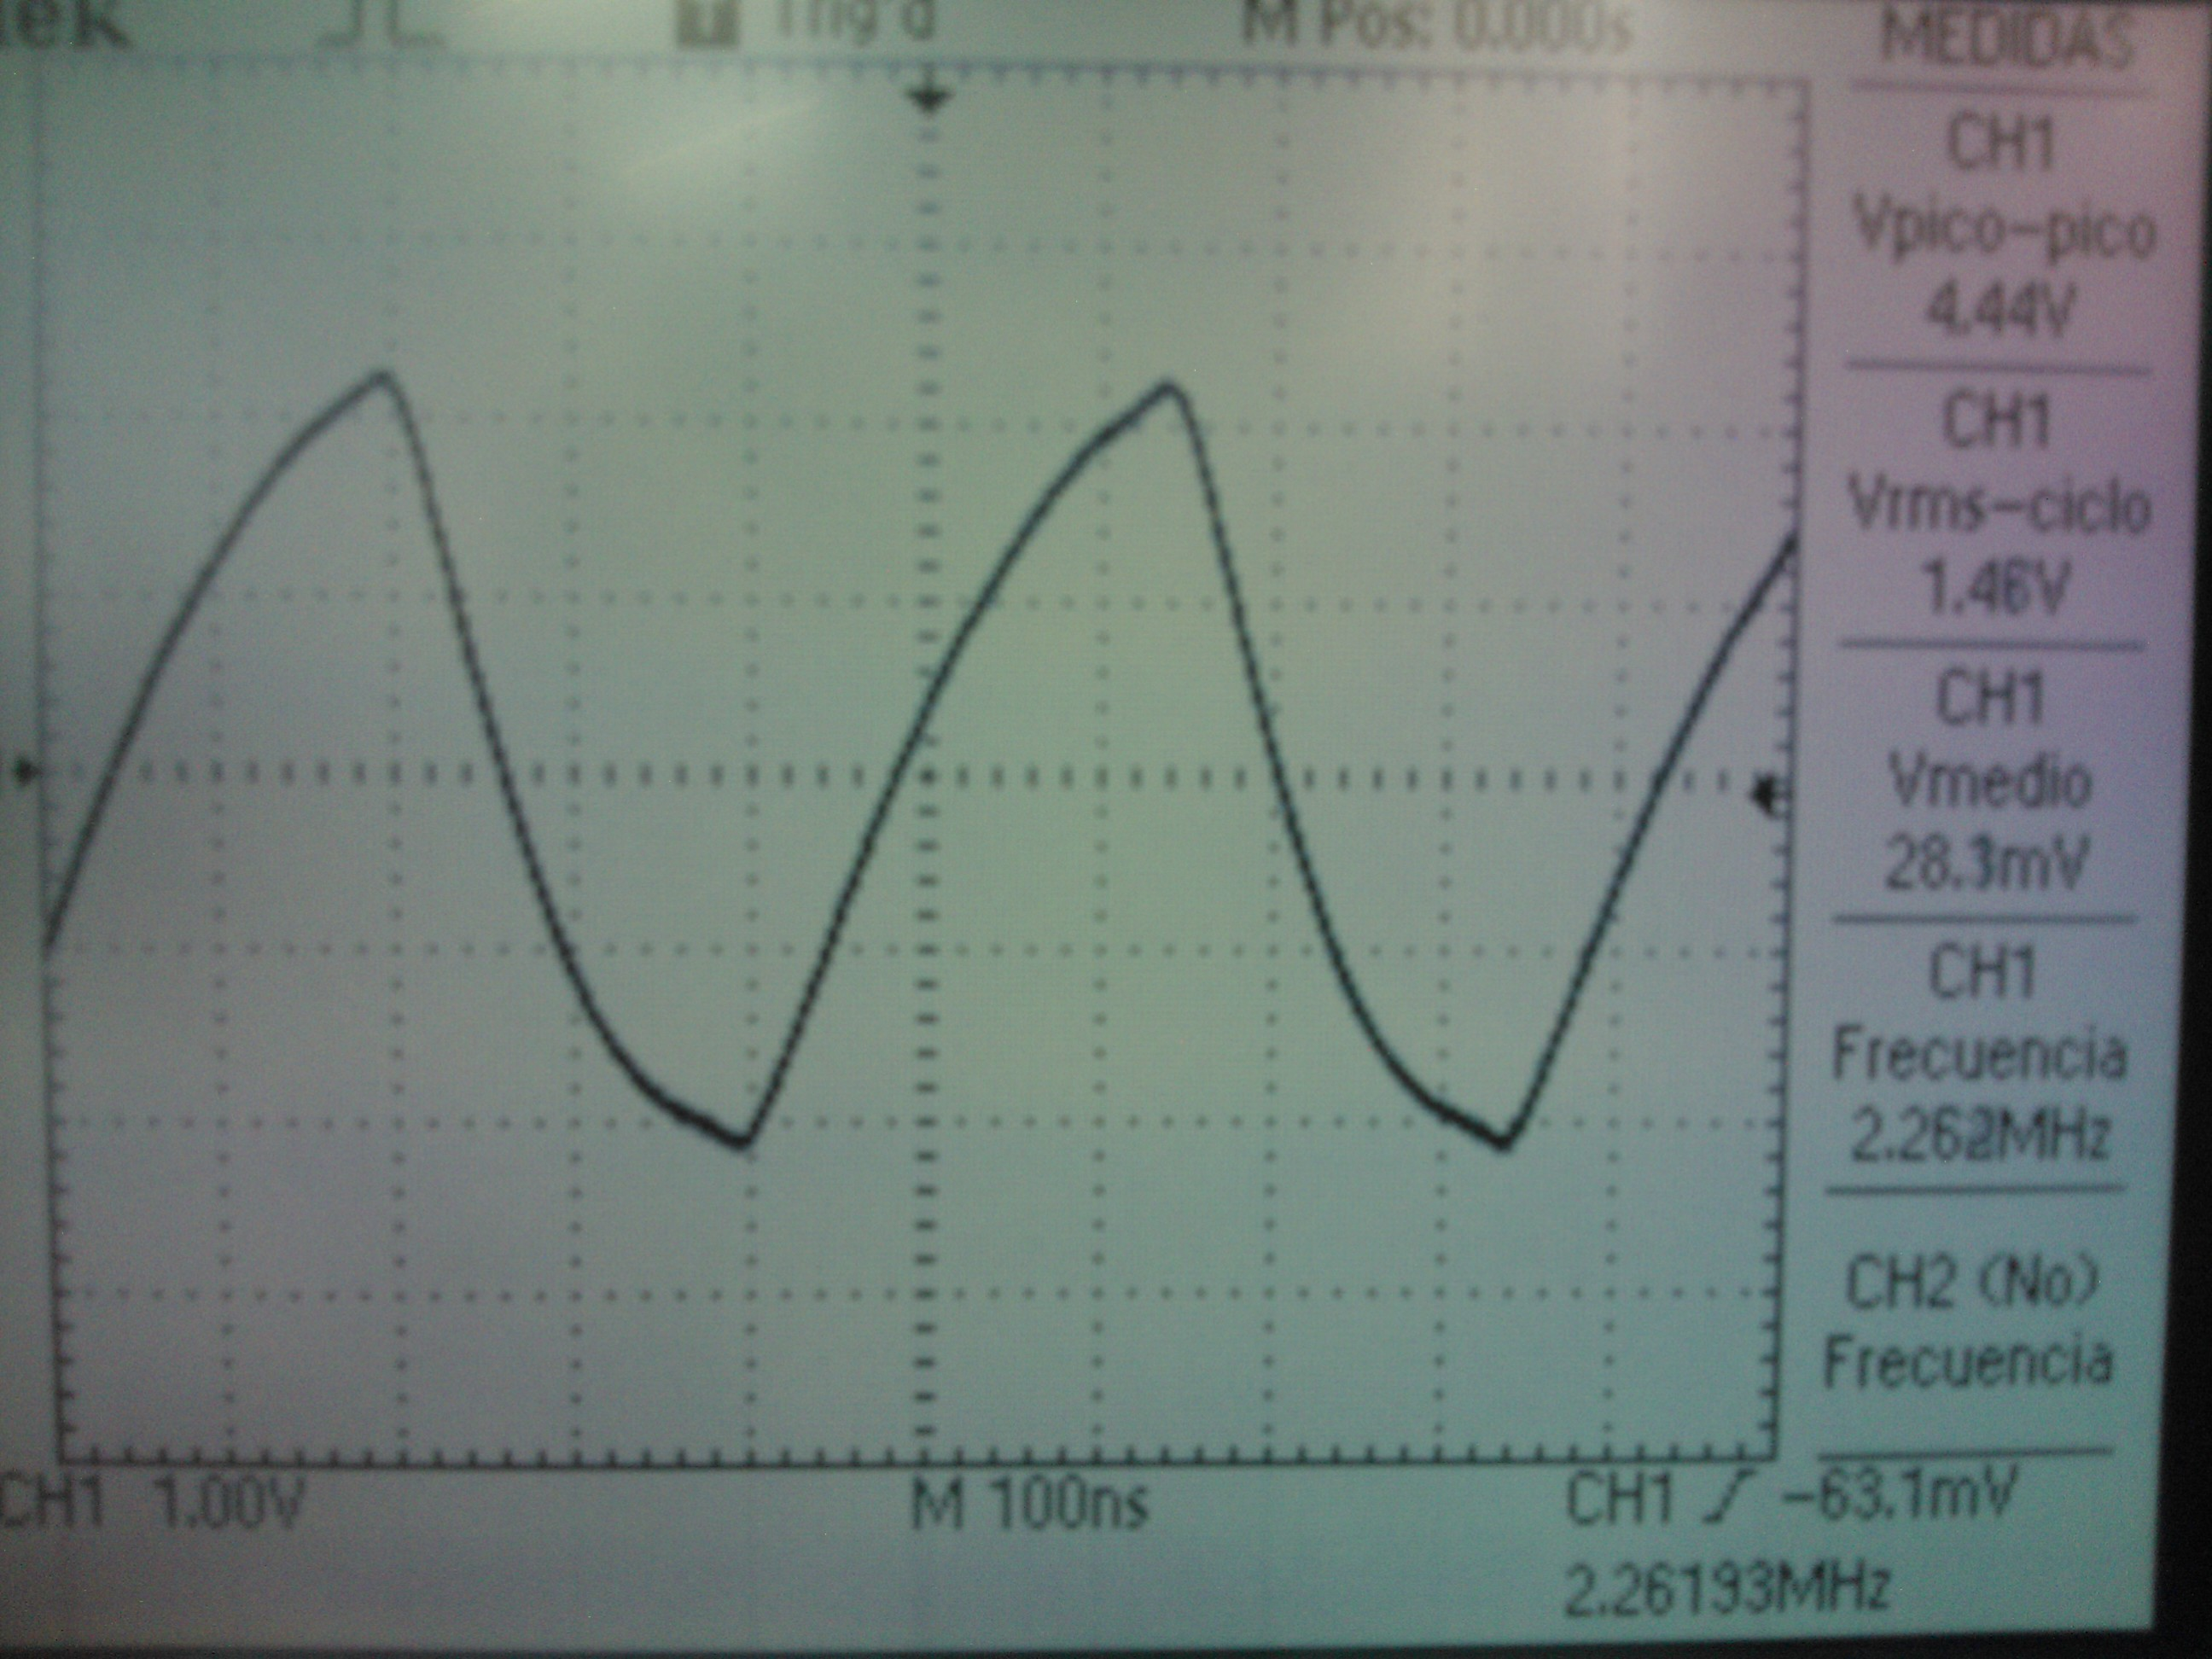
\includegraphics[width=0.40\textwidth]{./pics/WP_000051.jpg}
	\caption{Señal de salida para el oscilador en anillo con 7 negadores.}
	
	\label{anillo1}

\end{figure*}

\subsection{Oscilador controlado por voltaje.}
La configuración se probó para dos combinaciones diferentes de $R_1$ y $C_x$. 

\begin{itemize}
	%%%OJO, INFORMACIÓN POR COMPLETAR
	\item $R_1$ = 10 k$\Omega$ y $C_x$ = 1 nF. En este caso se tuvo $f_{min}=$ y $f_{max}=$ (ver figura~\ref{vco_1}).
	\item $R_1=$4.7 k$\Omega$ y $C_x=$10 nF. En este caso se tuvo $f_{min}=$6.21 kHz y $f_{max}=$7.73 kHz (ver figura~\ref{vco_2}).
\end{itemize}

En ambos casos se obtuvo una señal de salida más ``limpia'' para la frecuencia inferior de cada rango, es decir cuando en el transistor $V_{GS}<V_T$

%%%el el otro grafico f vs. VA lleva este label
% \label{vco_1}

\begin{figure*}[H]%[!t]
\centering
	%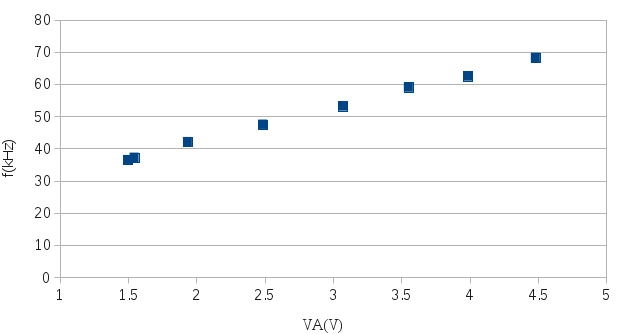
\includegraphics[width=0.45\textwidth]{./pics/vco_1.png}
	\caption{ Gráfica de frecuencia de salida $f$ vs. tensión de entrada $V_A$ para $R_1$=10 k$\Omega$ y $C_x$=1 nF.}
	
	\label{vco_1}

\end{figure*}

\begin{figure*}[H]%[!t]
\centering
	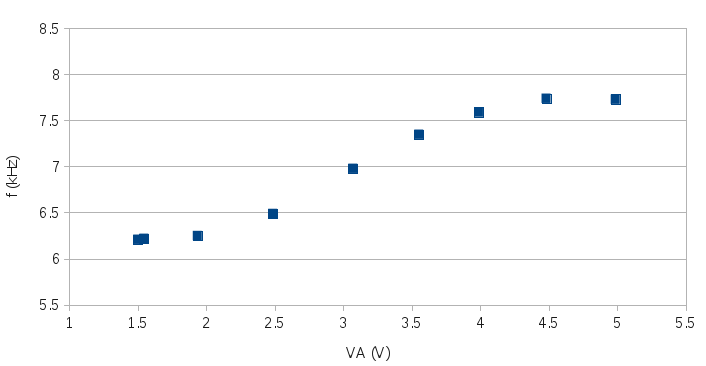
\includegraphics[width=0.45\textwidth]{./pics/vco_2.png}
	\caption{ Gráfica de frecuencia de salida $f$ vs. tensión de entrada $V_A$ para $R_1$=4.7 k$\Omega$ y $C_x$=10 nF.}
	
	\label{vco_2}

\end{figure*}

\section{Análisis y conclusiones.}

\subsection{Montaje y observación de osciladores.}
En el caso del oscilador de anillo, se tiene que la principal limitación es que dada una frecuencia de oscilación es difícil lograr una configuración que cumpla con dicha frecuencia, pues el circuito depende de los parámetros de tiempo de los transistores, que pueden variar notablemente respecto a los valores nominales. 

En el caso del VCO, se tiene como principal desventaja que la ganancia y la forma de onda obtenida a la salida es muy sensible a la variación de la tensión de entrada. Sin embargo, es sencillo obtener una frecuencia específica de oscilación variando la tensión de entrada y los valores de $R_1$ y $C_x$.


%\begin{figure*}[H]%[!t]
%\centering
%	\includegraphics[width=0.3\textwidth]{./f2d.png}
%	\caption{Circuitos usados para la caracterización de los transistores JFET (izq.) y MOSFET (der.). }
%	
%	\label{conf_jfet}
%
%\end{figure*}




%\begin{table}[!t]
%	%% increase table row spacing, adjust to taste
%	\renewcommand{\arraystretch}{1.1}
%	% if using array.sty, it might be a good idea to tweak the value of
%	 %\extrarowheight as needed to properly center the text within the cells
%	\caption{Parámetros de tensión medidos en ambos negadores.}
%	\label{t1}
%	\centering
%	%% Some packages, such as MDW tools, offer better commands for making tables
%	%% than the plain LaTeX2e tabular which is used here.
%	\begin{tabular}{|c||c||c|}
%	\hline
%	\bf Parámetro & \bf 74LS04 & \bf CMOS \\
%	\hline
%	
%	\end{tabular}
%\end{table}


% Can use something like this to pCaut references on a page
% by themselves when using endfloat and the captionsoff option.
%\ifCLASSOPTIONcaptionsoff
%  \newpage
%\fi


%%%%%%%%%%%%%% BIBLIOGRAF\'IA %%%%%%%%%%%%%%%%%%%
\begin{thebibliography}{1}

\bibitem{cd4007}
Fairchild Semiconductor. CD4007C -- Dual complementary pair plus inverter. \url{http://cva.stanford.edu/classes/cs99s/datasheets/CD4007C.pdf}



\end{thebibliography}

%\newpage
%%%%%%%%%%%%%%%%%% FIGURAS %%%%%%%%%%%%%%%%%%%%%


%\begin{figure*}[h]%[!t]
%\centering
%	\includegraphics[width=13cm]{./fig6a.png}
%	\caption{Controlador proporcional integral.}
%	
%	\label{parte2a}
%
%\end{figure*}


\end{document}

